\documentclass{bmvc2k}

%% Enter your paper number here for the review copy
\bmvcreviewcopy{853}


\usepackage{mathptmx} % assumes new font selection scheme installed
\usepackage{times} % assumes new font selection scheme installed
\usepackage{amsmath} % assumes amsmath package installed
\usepackage{amssymb}  % assumes amsmath package installed

\usepackage{array}

\usepackage{soul} % vahid: for cross out

\usepackage[T1]{fontenc}
\usepackage{color}
\usepackage{enumerate}
%\usepackage{caption}
\definecolor{red}{rgb}{1.00,0.00,0.00}
\definecolor{blue}{rgb}{0.00,0.00,1.00}
\definecolor{green}{rgb}{0.4,1.00,0.0}
\definecolor{yellow}{rgb}{0.5,0.5,0.0}
\newcommand{\cred}[1] {\textcolor{red}{#1}}
\newcommand{\cblue}[1] {\textcolor{blue}{#1}}
\newcommand{\cgreen}[1] {\textcolor{green}{#1}}
\newcommand{\cyellow}[1] {\textcolor{yellow}{#1}}

\usepackage{float}
%\usepackage{dblfloatfix}
\usepackage{graphicx} % for pdf, bitmapped graphics files
 \graphicspath{{./figures/}}
  % and their extensions so you won't have to specify these with
  % every instance of \includegraphics
 \DeclareGraphicsExtensions{.pdf,.jpg,.png}

\usepackage{xcolor}
\usepackage[export]{adjustbox}

%\usepackage{mwe,tikz}\usepackage[percent]{overpic}

%\usepackage[ruled,vlined]{algorithm2e}
%\usepackage{algorithmic,algorithm2e,float}
%\usepackage{algorithmicx}
%\usepackage[vlined]{algorithm2e}
\usepackage{listings}

\usepackage{algorithm}
\usepackage{algpseudocode}
\usepackage{setspace}

% useful packages for now
\usepackage{todonotes}

\algtext*{EndIf}% Remove "end if" text
\algtext*{EndWhile}% Remove "end while" text
\algtext*{EndFor}% Remove "end for" text
\algtext*{EndProcedure}% Remove "end procedure" text

% begin vertical rule patch for algorithmicx (http://tex.stackexchange.com/questions/144840/vertical-loop-block-lines-in-algorithmicx-with-noend-option)
\makeatletter
% start with some helper code
% This is the vertical rule that is inserted
\newcommand*{\algrule}[1][\algorithmicindent]{\makebox[#1][l]{\hspace*{.5em}\vrule height .75\baselineskip depth .25\baselineskip}}% 
\newcount\ALG@printindent@tempcnta
\def\ALG@printindent{%
    \ifnum \theALG@nested>0% is there anything to print
        \ifx\ALG@text\ALG@x@notext% is this an end group without any text?
            % do nothing
            \addvspace{-3pt}% FUDGE for cases where no text is shown, to make the rules line up
        \else
            \unskip
            % draw a rule for each indent level
            \ALG@printindent@tempcnta=1
            \loop
                \algrule[\csname ALG@ind@\the\ALG@printindent@tempcnta\endcsname]%
                \advance \ALG@printindent@tempcnta 1
            \ifnum \ALG@printindent@tempcnta<\numexpr\theALG@nested+1\relax% can't do <=, so add one to RHS and use < instead
            \repeat
        \fi
    \fi
    }%
\usepackage{etoolbox}
% the following line injects our new indent handling code in place of the default spacing
\patchcmd{\ALG@doentity}{\noindent\hskip\ALG@tlm}{\ALG@printindent}{}{\errmessage{failed to patch}}
\makeatother
% end vertical rule patch for algorithmicx

\renewcommand{\algorithmicrequire}{\textbf{Input:}}
\renewcommand{\algorithmicensure}{\textbf{Output:}}

\newtheorem{definition}{Definition}

% As of 2011, we use the hyperref package to produce hyperlinks in the
% resulting PDF.  If this breaks your system, please commend out the
% following usepackage line and replace \usepackage{icml2015} with
% \usepackage[nohyperref]{icml2015} above.
\usepackage{hyperref}

% Packages hyperref and algorithmic misbehave sometimes.  We can fix
% this with the following command.
%%\newcommand{\theHalgorithm}{\arabic{algorithm}}

\usepackage{amsmath}
 \DeclareMathOperator*{\argmax}{arg\,max}
\DeclareMathOperator*{\argmin}{arg\,min}

\usepackage{tabularx}



% \addtolength{\abovedisplayskip}{-1.2mm}

% \addtolength{\belowdisplayskip}{-1.2mm}

% \addtolength{\textfloatsep}{-2mm}

% \addtolength{\abovecaptionskip}{-1mm}

%\balance

%%%%%%%%%%%%%%%%%%%%%%%%

% my hyphenation rules

%\hyphenation{http://lars.mec.ua.pt/public/Media/mriem/ipm}
\hyphenation{se-ve-ral do-ne}

\usepackage{acronym}
%\acrodef{label}[short]{\textit{long form}}
%\renewcommand*\acsfont{\textit}
\renewcommand*{\acffont}[1]{\textit{#1}}
\renewcommand*{\acfsfont}[1]{\textnormal{#1}}


\title{Exploring Deep Structural Plasticity for Visual Recognition on Neuromorphic Architecture}

% Enter the paper's authors in order
% \addauthor{Name}{email/homepage}{INSTITUTION_CODE}
\addauthor{Gi Hyun Lim}{ghlim71@wku.ac.kr}{1,2}
\addauthor{Petrut A. Bogdan}{petrut.bogdan@manchester.ac.uk}{2}
\addauthor{Oliver Rhodes}{oliver.rhodes@manchester.ac.uk}{2}
\addauthor{Andrew G. D. Rowley}{Andrew.Rowley@manchester.ac.uk}{2}
\addauthor{Steve B. Furber}{steve.furber@manchester.ac.uk}{2}
\addauthor{Angelo Cangelosi}{angelo.cangelosi@manchester.ac.uk}{2}

% Enter the institutions
% \addinstitution{Name\\Address}
\addinstitution{
 Department of Artificial Intelligence Convergence,\\
 Wonkwang University,\\ 
 Iksan, Korea
}
\addinstitution{
 Department of Computer Science,\\ 
 University of Manchester,\\ 
 Manchester, UK
}

\runninghead{Lim et al.}{Deep structural plasticity}

% Any macro definitions you would like to include
% These are not defined in the style file, because they don't begin
% with \bmva, so they might conflict with the user's own macros.
% The \bmvaOneDot macro adds a full stop unless there is one in the
% text already.
\def\eg{\emph{e.g}\bmvaOneDot}
\def\Eg{\emph{E.g}\bmvaOneDot}
\def\etal{\emph{et al}\bmvaOneDot}

%-------------------------------------------------------------------------
% Document starts here
\begin{document}

\maketitle

\begin{abstract}
% Structural plasticity.
% Dynamic vision sensor cameras or Event-based vision sensors
% deep structural plasticity
% sparse coding.
% Neuromorphic architecture 1 M SpiNNaker.
% PyNN, SpyNNaker, pyDVS
Synaptic rewiring in the brain occurs throughout life. There is tight interplay between structural changes in the connectivity between neurons and the efficacy of existing connections. 
% Topographic organization allows optimal wiring between neurons, especially sensory connections to the central nervous system.
It has been found that topographic organization enables to achieve homeostasis for neuronal activity between regions, especially sensory connections to the central nervous system.
This work extends previous work done using a structural synaptic plasticity mechanism towards a biologically-inspired vision system. Accuracy of classification and speed of learning are evaluated by varying the number of hidden layers in the network. 
The system may learn the statistics of the inputs in an online fashion without supervision, pointing the way to engineered vision systems with similar online learning capabilities.
Moreover, we show the presented model can be used to classify handwritten digits by generating topographic maps between layers of neurons with small number of connections.
%The proposed approaches provides valuable insights to increase the performance of a neural circuit by increasing its scale in a structured manner.
The proposed approaches provides valuable insights to understand the phenomena of a neural circuit by increasing its scale in a structured manner.

%\todo[inline]{I've tried to re-word the abstract a bit. I bit more work could go into it to clearly outline the contribution of the paper.}
\end{abstract}

%-------------------------------------------------------------------------
%-------------------------------------------------------------------------
\section{Introduction}

The latest achievements in computer science, with massively parallel graphics processing units and large-scale neuromorphic hardware implementations such as SpiNNaker \cite{Furber2013}, and in cognitive robotics and neurorobotics, with the widespread use of robots such as iCub, provide the opportunity to significantly advance the understanding of human cognition and brains and to reach human-level artificial intelligence. 
%In November 2018 the world’s largest neuromorphic computing platform -- the 1 million ARM core SpiNNaker machine \cite{Furber2020}-- was switched on courtesy of the University of Manchester.
%The SpiNNaker machine has been designed and built to work in the same way a human brain does.
%The purpose to put the million cores into the machine makes it possible to simulate a billion biological neurons in real time.
%One billion neurons is just 1\% of the scale of the human brain but more than a whole mouse brain. 
The 1-million core SpiNNaker system has been in existence the world’s largest neuromorphic computing platform running in real time on custom digital multicore chips using the ARM architecture \cite{Furber2020}.
In practice the machine allows to simulate high-level real-time processing in a range of isolated brain networks such as 
an 80,000 neuron model of a segment of the cortex and the Basal Ganglia - an area affected in Parkinson’s disease.
However, there is still a wide disparity between the state-of-the-art artificial intelligence and human intelligence.
One of the missing links between them might be structural information that is how to represent the structure and the connectivity of the brain.
% The simple integration, on the other hand, is not enough to meet requirements in intelligent service robotics.
% We cannot rely only on the exponential increase in computing power to produce state of the art performance on a number of robotic tasks such as object/human behavior recognition and skill learning.

The structural and algorithmic properties of the neocortex provide an inspiration for computational architectures \cite{schmidhuber2015deep} such as Hierarchical Temporal Memory (HTM) \cite{Hawkins2004} and  Hierarchical Model (HMAX) \cite{Riesenhuber1999}.
They are computational models of the ventral stream of the visual cortex using a Bayesian belief revision algorithm and neural networks, respectively.
In reservoir computing (RC) which uses random connections within neural networks to map input signals into higher dimensional computational spaces \cite{Lukosevicius2009}, it has been reported that that the performance in a reservoir with small number of connections is equivalent to that in a reservoir with full connections.
The basic idea of RC architecture is to extend the sparse connectivity property in a hierarchical structured manner.
Just as layers in a deep neural network, modular reservoirs have been trained by using the outputs from directly connected reservoirs as input \cite{DeAzambuja2016a}.
Structural information that is a collection of spatial and temporal representations between entities present in the situation is used to help reduce the search space.
%% TODO:: the exponential distance rule (https://www.sciencedirect.com/science/article/pii/S0896627313006600)
The brain network with the two small-world properties, long-range connectivity and high clustering, seems to be developed n favor of more efficient wiring of connections \cite{Butz2014}. 
Thus, building maps between neural areas with a small number of connections is a key factor to understand the brain functions and structures.


Event-based vision sensors \cite{gray1989oscillatory} and a neuromorphic platform exemplified by the SpiNNaker machine \cite{Furber2020} has been used to organize receptive fields into a topographic map by synaptic rewiring or structural plasticity \cite{bogdan2018structural, hopkins2018spiking}.

We use this approach to explore structural synaptic plasticity in depth as a possible mechanism whereby biological vision systems may learn the statistics of their inputs without supervision, pointing the way to engineered vision systems with similar online learning capabilities \cite{garcia2016pydvs}.
% , pyDVS \cite{garcia2016pydvs}
Proposed deep structural plasticity is described using the PyNN \cite{davison2009pynn} which is a simulator-independent description language. 
sPyNNaker \cite{rhodes2018spynnaker} is the simulator that executes the specification on SpiNNaker. %\todo[inline]{PyNN is a simulator-independent description language. sPyNNaker is the simulator that executes the specification.}

%\todo[inline]{This is optional, but I think it focuses the paper. Here, I would also say where the results were good.}
The contribution of this work stands in its expansion of previous work using structural plasticity for the classification of handwritten digits. The previous input-output mapping was extended by adding multiple hidden layers, the effect of which is described in Section~\ref{section:results}. 
% This approach, while not yet yielding state-of-the-art results, provides valuable insights into an approach to increase the performance of a neural circuit by increasing its scale in a structured manner.
This approach, while not yet yielding state-of-the-art results, provides valuable insights into an approach to understand the phenomena of a neural circuit by increasing its scale in a structured manner.


%-------------------------------------------------------------------------
% \section{Retinotopic mapping}
% % \section{Topographic mapping for the visual pathways}
% Topographic mapping for the visual pathway
% synaptic rewiring

% \subsection{Lateral inhibition}
% winner takes all?

%% TODO: after inhibitory feed-forward
% \subsection{Difference of Gaussians}
% on and off bipolar cells

%% TODO: after lateral inhibition
% \subsection{Winner takes all networks?}


%-------------------------------------------------------------------------
\section{Related Work}
%\todo[inline]{I would rename this to Related Work, or simply not have an extra section (merging it into the introduction would be fine).}

\subsection{Synaptic plasticity}

A vital feature of the brain is its ability to learn and memorize something new. 
Consequently, there are changes not only of synaptic strength between connected neurons but also of the wiring pattern by modifying the connections in the intact adult brain \cite{albieri2015rapid}.
A neuronal topographic map represents topological relationships which imply projections from one brain area to another.

Alongside weight changes between neural connections, there are findings reporting that learning and memory  could involve alterations to the wiring diagram.
Dissimilar to weight changes, cortical rewiring relies on structural plasticity \cite{Chklovskii2004b}.
Structural plasticity in the form of synaptic rewiring is also a useful computational tool, used to automatically generate connectivity based on experimental activity data \cite{Diaz-Pier2016a}.
In consideration of development of topographic mappings in both synaptic weight change and synaptic formation and elimination, \cite{bamford2010synaptic} serves as a demonstration of the potential utility of synaptic rewiring as a means of prolonging the retention of learnt patterns.
From now on in the paper, the terms ''structural plasticity'' is used interchangeably with ''synaptic rewiring''.
Additionally, the term will be used to connote the meaning of changes in synaptic weights.

\subsection{Event-based neuromorphic systems}

Event-based systems are mostly composed of bio-inspired vision sensors and energy efficient neuromorphic computing systems. 
While traditional vision sensors capture the entire image at a fixed rate, event-based vision sensors (EVSs) respond relative changes in temporal contrast asynchronously \cite{Indiveri2015}.
%measure sufficient change in per-pixel brightness asynchronously \cite{Gallego2019}.
Vertebrate eyes provide inspiration to EVSs, in particular from the function of photoreceptors which react to changes in illumination.
By mimicking the structure and processing of the brain, neuromorphic platforms are massively parallel and energy efficient computing systems for spiking neural networks.
Since action potentials or spikes are inherently asynchronous events, an EVS can be coupled with a neuromorphic platform, because it is straightforward to convert visual events into spikes, and vice versa  \cite{Gallego2019}.

Numerous large-scale neuromorphic computing platforms have been emerged as a brain-inspired approach to information processing \cite{Thakur2018} such as IBM TrueNorth, Intel Loihi, BrainScaleS \cite{Schmitt2017a} and SpiNNaker.
The largest neuromorphic architecture - the 1 million core SpiNNaker machine has switched on courtesy of the University of Manchester \cite{Furber2020}. 
The SpiNNaker machine has been designed and built to work in the same way a human brain does. 
The purpose to put million cores into the machine is to make it possible to model a billion biological neurons in real time. 
One billion neurons are still only about 1\% of the scale of the human brain but more than a whole mouse brain.

The neuromorphic aspect of SpiNNaker is the way each core is connected to 6 of its neighbouring cores. 
Biological neural networks display very high degrees of connectivity, with neurons often having many thousands of inputs, sometimes as many as quarter of a million. 
Here, SpiNNaker network communications between cores uses small packets which borrows the well-established neuromorphic technique of address event representation (AER \cite{Mahowald1992}), wherein each neuron is given a unique numerical ‘address’ and the only information included in the packets is the source neuron information.

\subsection{Visual encoding}

Visual cortex is the core part of the cerebral cortex to process visual information \cite{katzner2009local}.
\cite{lee1998role} presents data that the primary visual cortex (area V1) seems to be involved in various higher level vision including the computation of cue-invariant boundaries, figure-ground distinction and the medial axis of shape.
% visual cortex \cite{gray1989oscillatory} \cite{katzner2009local} of higher level vision \cite{lee1998role}, \cite{grossberg2003does}
% topological representations \cite{kosslyn1995topographical}
% visual features \cite{eckhorn1990feature}
% cat visual cortex \cite{eckhorn1990feature}
% 3d vision \cite{grossberg19943}
% sensory coding \cite{field1994goal}\
Research during the past several decades on the functional architecture of the retina has found that the image projected onto the retina and captured by the photoreceptors is processed locally by sending a diverse set of parallel, highly processed images \cite{roska2014retina, Sanes2015}.

One of meaningful purposes of topographic maps may serve to perform dimension reduction, that they may have arisen through reasons of wiring efficiency \cite{bamford2010synaptic}.
% deep learning \cite{lecun2015deep} biologically inspired approaches \cite{bellec2019biologically}
% sparse connection \cite{Bellec2017}
% sparse coding \cite{olshausen1996emergence} 
% temporal coding \cite{engel1992temporal} 
Ganglion cells in mammalian retinas can serve to encode visual information into multiple representations using distinct features \cite{roska2014retina}, likely following a sparse coding scheme in which visual information is transformed to encode with a minimum number of active cells \cite{Field1994}.
There are also inhibitory connections from neighbouring cells in a layer. 
Their main roles of lateral inhibition are competition between different representations and stabilize the topographic mapping \cite{Kisvarday1994,mauss2015neural}.
% lateral inhibition has a homeostatic effect upon the network.
% lateral inhibition is the capacity of an excited neuron to reduce the activity of its neighbors. Lateral inhibition disables the spreading of action potentials from excited neurons to neighboring neurons in the lateral direction. This creates a contrast in stimulation that allows increased sensory perception.

%-------------------------------------------------------------------------
\section{Methods}
%\todo[inline]{I think the section should be called Methods, with a smaller sub-section called Model.}

\subsection{Deep Structural Plasticity}

With an event-based vision stream, pre-processing based upon a retinal model, and a suitable neuromorphic platform such as SpiNNaker, we can then proceed to perform additional processing to achieve outcomes such as object recognition and classification. In the following sections, we discuss some of the principles of visual processing in the brain, and some experimental work to develop object classification systems based upon those principles.

Bamford et al. \cite{bamford2010synaptic} proposed the model of synaptic rewiring between two layers. 
Where each neuron in the source layer innervates neurons in the target layer, the mapping between the layers is supposed to be topographically arranged as neighbouring neurons in the target layer are responsive to the activity of neighbouring neurons in the source layer \cite{udin1988formation} through the mechanism of homeostasis \cite{Butz2009}. 
The model has been implemented in the context of a structural plasticity framework on SpiNNaker, operating in real time in parallel by activity-independent and/or activity-dependent processes \cite{bogdan2018structural}.
In line with their implementation, it is extended in depth by adding hidden layers between the source and target layers, as shown in Fig. \ref{fig:dsp}, and continues to analyze the characteristics of the model by applying it to a discrimination task: handwritten digit classification \cite{hopkins2018spiking}.

\begin{figure}[tbh]
    \centering
    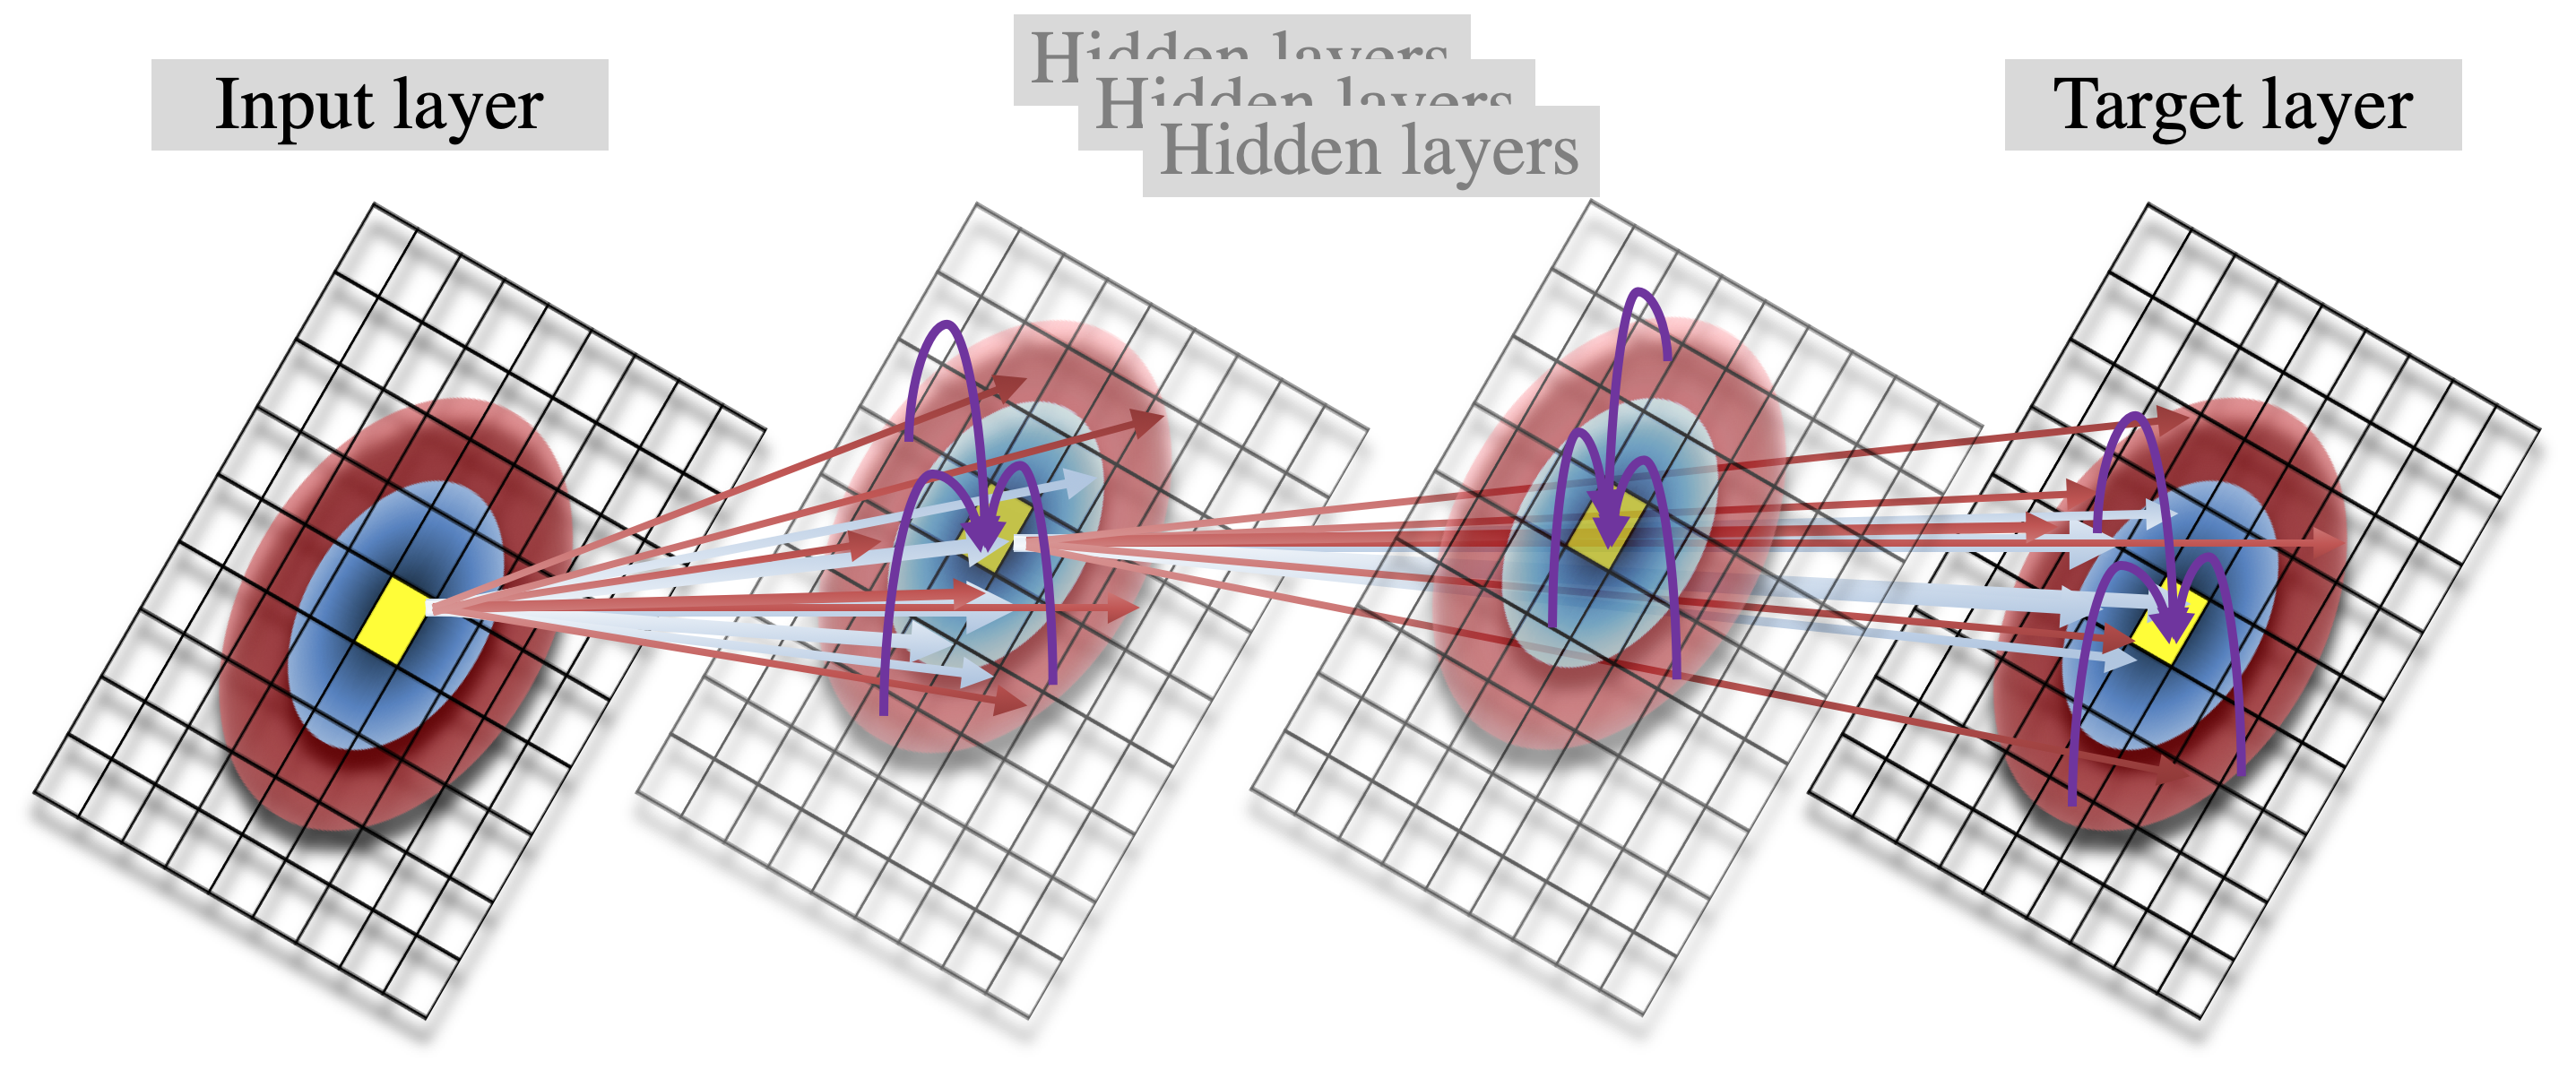
\includegraphics[width=0.70\linewidth, trim=0cm 0cm 0cm 0cm, clip=true]{DSP_n}
    \caption{Deep structural plasticity for topographic mapping}
    \label{fig:dsp}
\end{figure}

\subsection{Model}
The mammalian retina encodes visual information into multiple representations using distinct features \cite{roska2014retina}. 
The principle of encoding is to represent all the likely inputs with a relatively small number of neurons with minimal loss in decoding of the input \cite{field1994goal}. 

In the source layer of our visual encoding model, there are feed-forward connections from the photoreceptors to the receptive fields which have a spatial structure to transmit the input and pass it on to the following layer.
Feed-forward weights are computed according to the photoreceptor array with a two-dimensional Gaussian kernel ($\mathbf{W}_F$) as a convolution which can be described as the difference between two circularly symmetric Gaussian functions.
% a center-surround receptive field or DoG
% Here, the main mechanism for this encoding is competition between different representations through lateral inhibition from neighbours in the following layer.
Lateral inhibition from neighbours in the following layer which leads competition between different representation should be the main mechanism for this encoding.
The weights for inhibitory connections are computed by the cross-correlation of the input kernels, 
%\todo[inline]{Where/how are you doing this in your experiments? The difference between Case 2 and 3 is wo/w lateral inhibition.}
%
\begin{equation}
    \mathbf{W}_{L}  = \mathbf{W}_{F1} \ast \mathbf{W}_{F2} ,
\end{equation}
%
where $\ast$ denotes the convolutional operation between two functions.
%% TODO:: more comment
Those feed-forward and lateral connections are normalized and so that they sum to one, and scaled by the required weight so that a single spike will activate the characterized neuron in the following layer; 
this has the effect of distributing the required activity across the entire receptive field. 
By computing weights in this manner, neighbours will be inhibited proportionally to the similarity of the regions they represent. 
In each layer ($i$), their computed weights ($\mathbf{W}_L^i$) for lateral inhibitory connections can be considered negative, which means that the total computation ($\mathit{f}_G^i$) of the circuit can act as a centre-surround filter:
%
\begin{equation}
%    \mathit{f}_G^i  \varpropto \mathit{f}^i_{F}(\mathbf{W}^i_{F}) - \mathbf{W}_{L}^i .
    \mathit{f}_G^i  \propto \mathit{f}^i_{F}(\mathbf{W}^i_{F}) - \mathbf{W}_{L}^i .
\end{equation}
%
The computation continues up to the target layer through hidden layers.

The competition in each afferent layer produces a temporal code in which each spike represents a region of the input whose activity matches the receptive field of the spiking neuron quite closely.
% The receptive fields can be viewed as bases of a vector space; although the bases are not orthogonal, competition will push the representation towards orthogonality.
Additionally, the inhibition of neurons representing similar inputs, and the consequent reduction of output spike activity, creates a sparse representation that should provide subsequent stages of the visual pipeline with patterns that are easier to separate.


\subsection{Topographic mapping}

Bamford et al. \cite{bamford2010synaptic} introduced two probabilistic rules for synaptic rewiring: one for synaptic formation, the other for elimination.
Rewiring relies on uniform sampling over all potential synapses. 
Formation is a probabilistic, activity-independent
%\todo[inline]{Which formation rule are you using? There are 2 formation rules currently implemented: activity-dependent (most recent neuron to have fired is considered a partner for formation) and activity-independent (sampling randomly from possible pre-synaptic partners).: comparison between Case 1 & Case 3} 
process which randomly selects a pre- and postsynaptic neuron to establish whether a connection between the two exists by taking into account the distance $\delta$ between candidate neurons. 
A new synapse is formed with maximum weight $g_{max}$ if
%
\begin{equation} \label{eq:formation_rule}
r<p_{form}e^{-\frac{\delta^2}{2\sigma^2_{form}}},
\end{equation}
%
where $r$ is a uniform random number in the interval $[0, 1)$, $p_{form}$ is the peak formation probability, and $\sigma^2_{form}$ is the variance of the connection field, or the spread of the region of preferential connections.

The elimination rule states that if the synapse's conductance is less than half of the maximum allowed conductance, $0.5g_{max}$, it is eliminated with probability $p_{elim-dep}$, otherwise the probability $p_{elim-pot}$ is used.

If the randomly selected synaptic element exists, the removal rule is followed.
Removal is either carried out with a fixed probability $p_{elim-pot}$ when weights are static, or with a choice of $p_{elim-pot}$  or $p_{elim-dep}$ when applied in conjunction with spike-timing dependent plasticity (STDP \cite{Song2000}). 
Thus, a synapse is removed if
%
    %TODO:: something....
\begin{equation} \label{eq:elimination_rule}
\begin{aligned}
r<p_{elim}, \text{where }  p_{elim} = 
    \begin{cases}
        p_{elim-dep} \text{ for }   w_{syn}  < \theta_g \\
        p_{elim-pot} \text{ for }   w_{syn}  \geq \theta_g \\
    \end{cases},
\end{aligned}
\end{equation}
%
where $r$ is a random number sampled from a uniform distribution in the interval $[0, 1)$, $p_{elim-dep}$ is the elimination probability used when a synapse is depressed, $p_{elim-pot}$ is the elimination probability used when a synapse is potentiated, $w_{syn}$ is the weight of the synapse under consideration for removal and a weight threshold $\theta_g$ is selected as half of the maximum allowed weight ($ \theta_g = g_{max}$). 
If STDP is not presented in the simulated network, only $p_{elim-pot}$ is used as all synapses would have a fixed weight, namely $g_{max}$.

%Neurons within each afferent layer which is directly connected with feed-forward connections also receive lateral connections. \todo[inline]{I would rephrase to: Neurons in each layer receive both feed-forward connections as well as lateral, recurrent ones.}
Neurons in each layer receive both feed-forward connections as well as lateral, recurrent ones.
These are inhibitory and the main purpose in the network is to limit the spiking activity within the afferent layer. 
Lateral inhibition also has the effect of encouraging diversity of feature selection in the neuron population.
%\todo[inline]{Lateral inhibition also has the effect of encouraging diversity of feature selection in the neuron population. For example, not all neurons will respond to vertical bars as nearby neighbours are likely to already have captured that feature of the input, so some neurons will respond to vertical bars, while others will respond to horizontal ones.}
% While connections within each afferent layer abound, there are none between the layers.
Lateral connections are formed by the same means as feed-forward connections, though $\sigma_{form}$ can be different for each projection.

While dendritic spines in the real brain have been imaged extending and retracting over periods of hours compared with others stable over a month or more \cite{Grutzendler2002}, 
much higher rewiring rates have been used in the simulations so that synapses had several chances to rewire during the short periods for which it was tractable to run simulations.
The value of $p_{form}$ works together with the rewiring rate ($f_{rew}$), the number of synapses, $\sigma_{form}$, and the topology of the area to define the actual rate of formation.
$\sigma_{form-ff}$ (i.e. for feed-forward synapses) was given a larger value than $\sigma_{form-lat}$ (i.e. for lateral synapses), in line with generic parameters given by \cite{miikkulainen2006computational}.
Since $\sigma_{form-ff} > \sigma_{form-lat}$, $p_{form-ff}$ should be less than $p_{form-lat}$ in order to balance the overall probability of synapse formation with each afferent layer, to achieve this balance:
\begin{equation}
    p_{form-ff} = p_{form-ff} \frac{\sigma^2_{form-lat}}{\sigma^2_{form-lat}}.
\end{equation}
The mean formation rate can then be calculated. 
$p_{elim-dep}$ and $p_{elim-pot}$ were set at much lower than mean formation rates, so that the majority of the potential synapses would be formed at any point.

The proposed model is described using the PyNN \cite{davison2009pynn} simulator independent network description language. 
The SpiNNaker, simulator-dependent, implementation of PyNN (sPyNNaker \cite{rhodes2018spynnaker}) has been extended to perform synaptic rewiring. 
The same parameters in \cite{bogdan2018structural} have been used in the simulations.
%Table \ref{tab:sim_params} contains the parameters used in the simulations.

%\setlength{\tabcolsep}{4pt}
%\begin{table*}
%\setlength{\tabcolsep}{18pt} % Default value: 6pt
%\begin{center}
%\caption{The parameters used in the simulations}
%\label{tab:sim_params}
%\begin{tabular}{llll}
%\hline\noalign{\smallskip}
%    wiring & inputs & membrane & STDP \\
%\noalign{\smallskip}
%\hline
%\noalign{\smallskip}
%    $N_{layer}=28\times28$ 	& $f_{mean}=5$Hz 	& $v_{rest} = -70$mV 	& $A_{+} = 0.1$ \\
%    $S_{max}=96 $ 			& $t_{stim}=200$ms 	& $e_{ext} = 0$mV  		& $B = 1.2$	   \\
%    $\sigma_{form-ff}=5$		& ~ 			& $v_{thr} = -54$mV 		& $\tau_{+} = 20$ms \\
%    $\sigma_{form-lat}=5$ 		& ~ 			& $g_{max} = 0.2$Siemens& $\tau_{-} = 64$ms \\
%    $p_{form-ff}=0.16$ 		    & ~  			& $\tau_{m}=20$ms  		& ~ \\
%    $p_{form-lat}=1$ 			& ~  			& $\tau_{ex}=5$ms 		& ~ \\
%    $p_{elim-dep}=0.0245$		& ~  			& ~                     & ~ \\
%    $p_{elim-pot}=1.36 e -4$ 	& ~  			& ~	                    & ~ \\
%    $f_{rew}=10$ kHz			& ~  			& ~                     & ~ \\
%\hline
%\end{tabular}
%\end{center}
%\end{table*}
%\setlength{\tabcolsep}{1.4pt}

%\begin{table}
%    \centering
%    \caption{Topographic map formation model parameters}
%    \label{tab:synaptogenesis_parameters}
%    \begin{tabular}{|c|}
%        \hline
%        Wiring \\
%        \hline	
%        Size of layer = $16 \times 16$ \\
%        \hline
%        $S_{max} = 32$ \\
%        \hline
%        $ \sigma_{form\_feedforward} = 2.5$ \\
%        \hline
%        $ p_{form\_feedforward} = 0.16$ \\
%        \hline
%        $ \sigma_{form\_lateral}=1 $ \\
%        \hline
%        $ p_{form\_lateral} = 1 $ \\
%        \hline
%        $  p_{elim\_dep} = 0.0245$ \\
%        \hline
%        $  p_{elim\_pot} = 1.36e^{-4}$ \\
%        \hline
%        $ f_{rew} = 10^4 Hz $ \\
%        \hline
%    \end{tabular}
%%	\caption*{}
%	
%\end{table}


%\subsection{Computation model}

%\begin{algorithm}[h!]
%    \KwData{Parameters defined in Table \ref{tab:sim_params} and relevant probability LUTs.}
%    \KwResult{Three possible outcomes: a formed connection, a removed connection or no change to connectivity.}
%    \textbf{Initialisation:} copying rewiring parameters from SDRAM into DTCM, setting up data structures\;
%%    \dotfill\\
%\SetKwFunction{FMain}{timer\_callback}
%\SetKwProg{Fn}{function}{:}{}
%\Fn{\FMain{time}}{
%    \eIf{time passed since last rewiring attempt = rewiring period}{
%        Select arbitrary \textbf{post-synaptic\_id} using shared seed\;
%        \If{\textbf{NOT} lowest\_id\_on\_core  $\leq$ \textbf{post-synaptic\_id} $<$ highest\_id\_on\_core}{
%            \KwRet false\;
%        }
%        \tcc{All following random number generators use a local seed, as opposed to the shared seed used for synchronization.}
%        Select arbitrary synaptic slot\;
%        \eIf{synaptic slot \textbf{contains} an element}{
%            recover identifying information for pre-synaptic partner from synaptic slot element\;
%        }{
%        recover identifying information of the last neuron to have spiked\;
%    }
%    \
%    Queue DMA read request synaptic\_row based on SDRAM address of selected pre-synaptic id\;
%    \KwRet true\;
%}{
%    \KwRet false\;}
%}
%%\dotfill\\

%\SetKwFunction{FMain}{dma\_read\_callback}
%\SetKwProg{Fn}{function}{:}{}
%\Fn{\FMain{}}{
%	\eIf{selected \textbf{post-synaptic\_id} exists in synaptic\_row}{
%		elimination\_rule()\;
%	}{
%		formation\_rule()\;
%	}
%}
%%\dotfill\\

%\SetKwFunction{FMain}{formation\_rule}
%\SetKwProg{Fn}{function}{:}{}
%\Fn{\FMain{}}{
%	r=RNG(0, 1)\;
%	\eIf{$r < p_{form}e^{-\frac{\delta^2}{2\sigma_{form}^2}}$}{
%		Queue DMA write request to write the row back into SDRAM\;
%		\KwRet true\;
%	}{
%	\KwRet false\;
%	}
%}
%%\dotfill\\
%%\tcc{Elimination rule}

%\SetKwFunction{FMain}{elimination\_rule}
%\SetKwProg{Fn}{function}{:}{}
%\Fn{\FMain{}}{
%	r=RNG(0, 1)\;
%	\uIf{$synaptic\_weight < 0.5 g_{max}$ and $r < p_{elim-dep}$}{
%		Queue DMA write request to write the row back into SDRAM\;
%		\KwRet true\;
%	}
%	\uElseIf{$synaptic\_weight \geq 0.5 g_{max}$ and $r < p_{elim-pot}$}{
%		Queue DMA write request to write the row back into SDRAM\;
%		\KwRet true\;
%	}
%	\Else{
%		\KwRet false\;}
%}
%\caption{Algorithmic description of synaptic rewiring model running on SpiNNaker. A  load-time data structure set up is followed by the execution of the rewiring algorithm driven by timer callbacks. Individual formation or removal rules are considered only once the relevant synaptic row is brought into core-local memory from off-chip memory (SDRAM) through a DMA call.}
%\label{alg:synaptogenesis_c}

%\end{algorithm}

% \subsection{Neural dynamics}

% \subsection{Quality of topographic map}
% To analyse the quality of topographic map, the measures defined from \cite{bamford2010synaptic}: the spread of the mean receptive field $\sigma_{aff}$ and the Absolute Deviation ($AD$) of the mean receptive field from its ideal location are used.   
% The former relies on the search for the location around which afferent synapses have the lowest weighted variance $\sigma^2_{aff}$. 
% This is a move away from the centre of mass measurement used from \cite{Elliott1999} for identifying the preferred location of a receptive field. As a result, the centre of the receptive field that is being examined is the location that minimises the weighted standard deviation, computed as follows:
% %
% \begin{equation}
%     \sigma_{aff} = \sqrt{\frac{\sum_i{w_i\lvert{\vec{p}_{xi}}\rvert^2}}{\sum_i{w_i}}}
% \end{equation}
% %
% where $i$ loops over synapses, $x$ is a candidate preferred location, $\lvert{\vec{p}_{xi}}\rvert$ is the minimum distance from the location of the afferent for synapse $i$, and $w_i$ is the weight of the synapse.
% The candidate preferred location $x$ has been implemented with an iterative search over each whole number location in each dimension and then a further iteration to locate the preferred location to $1/10$th of a unit of distance. Thus, the preferred location $\vec{x}$ of a receptive field is given by the function: $\arg\min_{\vec{x}}{\sigma^2_{aff}}$.

% Once the preferred location of each neuron is computed, taking the mean distance from the ideal location of each preferred location results in a mean $AD$ for the projection. 
% We report both mean $AD$ and mean $\sigma_{aff}$ computed with and without taking into account connections and  weights. 
% $\sigma_{aff-weight}$ and $AD_{weight}$ are computed using synaptic weights $g_{syn}$, 
% while $\sigma_{aff-conn}$ and $AD_{conn}$ are designed to consider the effect of rewiring on the connectivity, thus synaptic weights are considered unitary.


% \subsection{Structural plasticity for classification}
By using topographic maps for a retinal model and visual pathways, the proposed model can be applied to achieve outcomes such as object recognition and classification on a suitable neuromorphic platform such as SpiNNaker.
The following sections present experimental work as an event-based vision system which can classify handwritten digits based on deep structural plasticity.

%-------------------------------------------------------------------------
\section{results}\label{section:results}
%\todo[inline]{I would rename this section results and move some of the descriptions of methods into the methods section.}

%\todo[inline]{``explore the characteristics of structural plasticity in depth'' means the same thing as ``fully explore the characteristics of structural plasticity'': I'm not sure only depth is full exploration}
To verify the proposed networks and explore the characteristics of structural plasticity in depth, the MNIST dataset is used. 
The MNIST dataset is a large database of $28 \times 28$ handwritten digits that is commonly used for training various image processing systems. 
These image sequences are converted using a Neuromorphic Vision Sensor emulator (pyDVS) \cite{garcia2016pydvs}.
the 3 considered cases: STDP in conjunction with synaptic rewiring (Case 1) and synaptic rewiring only without or with lateral connections (Case 2 and 3, respectively).

\begin{figure}[tbh]
    \centering
    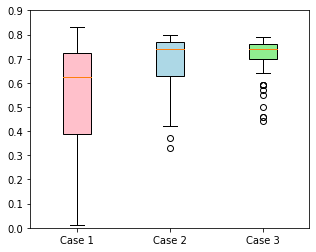
\includegraphics[width=0.70\linewidth, trim=0cm 0cm 0cm 0cm, clip=true]{10trials/boxPlotCase}
    \caption{Classification performance with respect to 3 cases}
    \label{fig:bpWCases}
\end{figure}

Figure \ref{fig:bpWCases} shows the performance of all the simulations for MNIST classification.
Simulations were performed on the 1 million SpiNNaker \cite{brown2018spinnaker} with three combinational settings for the classification of ten kinds of handwritten digits: three cases (Case 1-3), number of hidden layers (0-3 hidden layers) and four different training \& testing time ($300$s, $600$s, $900$s and $1,200$s) for 10 digit classes. 
The performance is measured from 10 trials of the combinatorial setting, thus total $10 \times 10 \times 3 \times 4 \times 4 = 4,800$ simulations each for training and testing. 
As per Fig. \ref{fig:bpWCases} and Table \ref{tab:sim_stat}, the best performance has been achieved in the Case 1 while the Case 3 shows the best average performance and the smallest variance. 

\setlength{\tabcolsep}{4pt}
\begin{table}
\setlength{\tabcolsep}{12pt} % Default value: 6pt
\begin{center}
\caption{The statistics of MNIST classification}
\label{tab:sim_stat}
\begin{tabular}{ llll }
\hline\noalign{\smallskip}
     ~          & Case 1    & Case 2    & Case 3    \\ 
\noalign{\smallskip}
\hline
\noalign{\smallskip}    
    Best 	    & 0.83	    & 0.8 	    & 0.79      \\ %from 84
    Average 	& 0.56031	& 0.68888 	& 0.72275   \\ %from 56
    Variance 	& 0.04929	& 0.01116	& 0.00381   \\ %from 72
\hline
\end{tabular}
\end{center}
\end{table}
\setlength{\tabcolsep}{1.4pt}

%-------------------------------------------------------------------------
\section{Discussion}
% 
%------------------------------------------------------------------------

\setlength{\tabcolsep}{4pt}
\begin{table}
\setlength{\tabcolsep}{12pt} % Default value: 6pt
\begin{center}
\caption{The best performances on MNIST classification}
\label{tab:sim_best}
\begin{tabular}{ llll }
\hline\noalign{\smallskip}
     ~          & Case 1    & Case 2    & Case 3    \\ 
\noalign{\smallskip}
\hline
\noalign{\smallskip}    
    0 hlayer 	& 0.83	    & 0.8	    & 0.79   \\
    1 hlayers 	& 0.71  	& 0.78   	& 0.78   \\
    2 hlayers	& 0.64  	& 0.76  	& 0.75   \\
    3 hlayers 	& 0.43  	& 0.63  	& 0.71   \\
\hline
\end{tabular}
\end{center}
\end{table}
\setlength{\tabcolsep}{1.4pt}

Table \ref{tab:sim_best} shows that simply adding hidden layers does not improve performance. Any result with hidden layers has not outperformed the baseline which have been achieved from the previous work \cite{hopkins2018spiking} without a hidden layer.
%\todo[inline]{It would be interesting to figure out why this is the case? Is the firing rate going down with each subsequent layer, thus preventing accurate classification? Are the hidden layers learning anything new from the previous layer?}

\begin{figure*}[tbh]
    \centering
    \begin{centering}
    \begin{tabular}{ccc}
        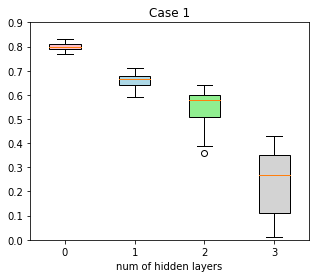
\includegraphics[width=0.30\linewidth, trim=0cm 0cm 0cm 0.65cm, clip=true]{10trials/boxPlotHlayersC1}&
        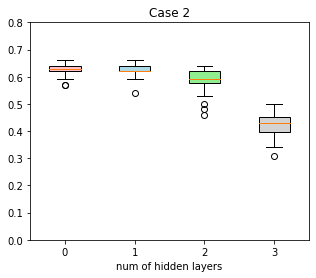
\includegraphics[width=0.30\linewidth, trim=0cm 0cm 0cm 0.65cm, clip=true]{10trials/boxPlotHlayersC2}&
        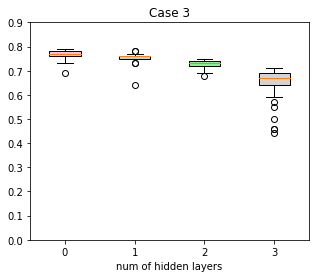
\includegraphics[width=0.30\linewidth, trim=0cm 0cm 0cm 0.65cm, clip=true]{10trials/boxPlotHlayersC3}\\
        Case 1 & Case 2 & Case 3
        \end{tabular}
     \end{centering}
     \caption{Classification performance with respect to three cases}
     \label{fig:bpTtime}
    \vspace{-10pt}
\end{figure*}

Figure \ref{fig:bpTtime} shows the performance over training time for each case. While the best averaged and stable results have been produced at the Case 3, the best result was delivered without hidden layer at the Case 1. 
However, simultaneous operation of STDP and rewiring in the presence of correlated input requires more training time as adding more hidden layers.

\begin{figure*}[tbh]
    \centering
    \begin{centering}
    \begin{tabular}{ccc}
        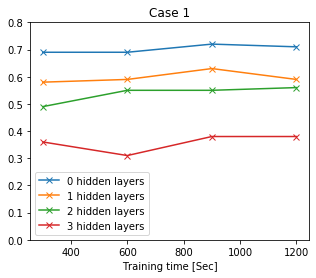
\includegraphics[width=0.30\linewidth, trim=0cm 0cm 0cm 0.65cm, clip=true]{10trials/evolMaxC1}&
        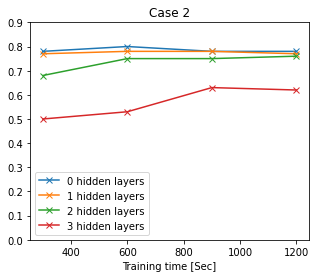
\includegraphics[width=0.30\linewidth, trim=0cm 0cm 0cm 0.65cm, clip=true]{10trials/evolMaxC2}&
        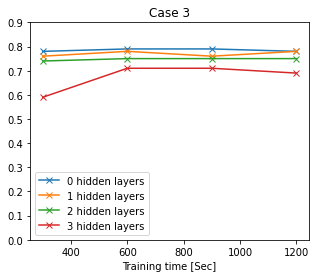
\includegraphics[width=0.30\linewidth, trim=0cm 0cm 0cm 0.65cm, clip=true]{10trials/evolMaxC3}\\
        Case 1 & Case 2 & Case 3
        \end{tabular}
     \end{centering}
     \caption{Evolution of the best classification performance}
     \label{fig:evHlayerBest}
    \vspace{-10pt}
\end{figure*}

\begin{figure*}[tbh]
    \centering
    \begin{centering}
    \begin{tabular}{ccc}
        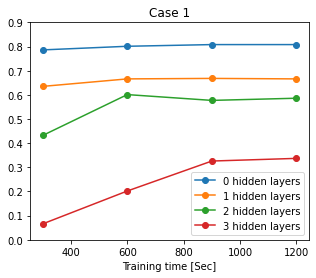
\includegraphics[width=0.30\linewidth, trim=0cm 0cm 0cm 0.65cm, clip=true]{10trials/evolAvgC1}&
        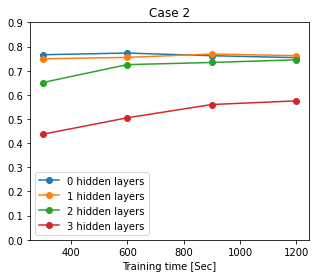
\includegraphics[width=0.30\linewidth, trim=0cm 0cm 0cm 0.65cm, clip=true]{10trials/evolAvgC2}&
        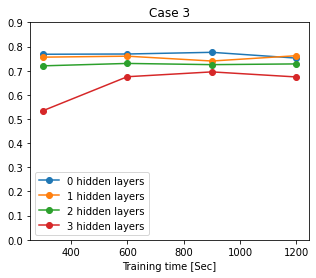
\includegraphics[width=0.30\linewidth, trim=0cm 0cm 0cm 0.65cm, clip=true]{10trials/evolAvgC3}\\
        Case 1 & Case 2 & Case 3
        \end{tabular}
     \end{centering}
     \caption{Evolution of the average classification performance}
     \label{fig:evHlayerAvg}
    \vspace{-10pt}
\end{figure*}

Figure \ref{fig:evHlayerBest} and \ref{fig:evHlayerAvg} show the evolution of the best and average classification performance with respect to the cases, respectively. 
In the case of synaptic rewiring without STDP (Case 3), there is no significant difference in performance regarding the number of hidden layers.

\begin{figure*}[tbh]
    \centering
    \begin{centering}
    \begin{tabular}{ccc}
        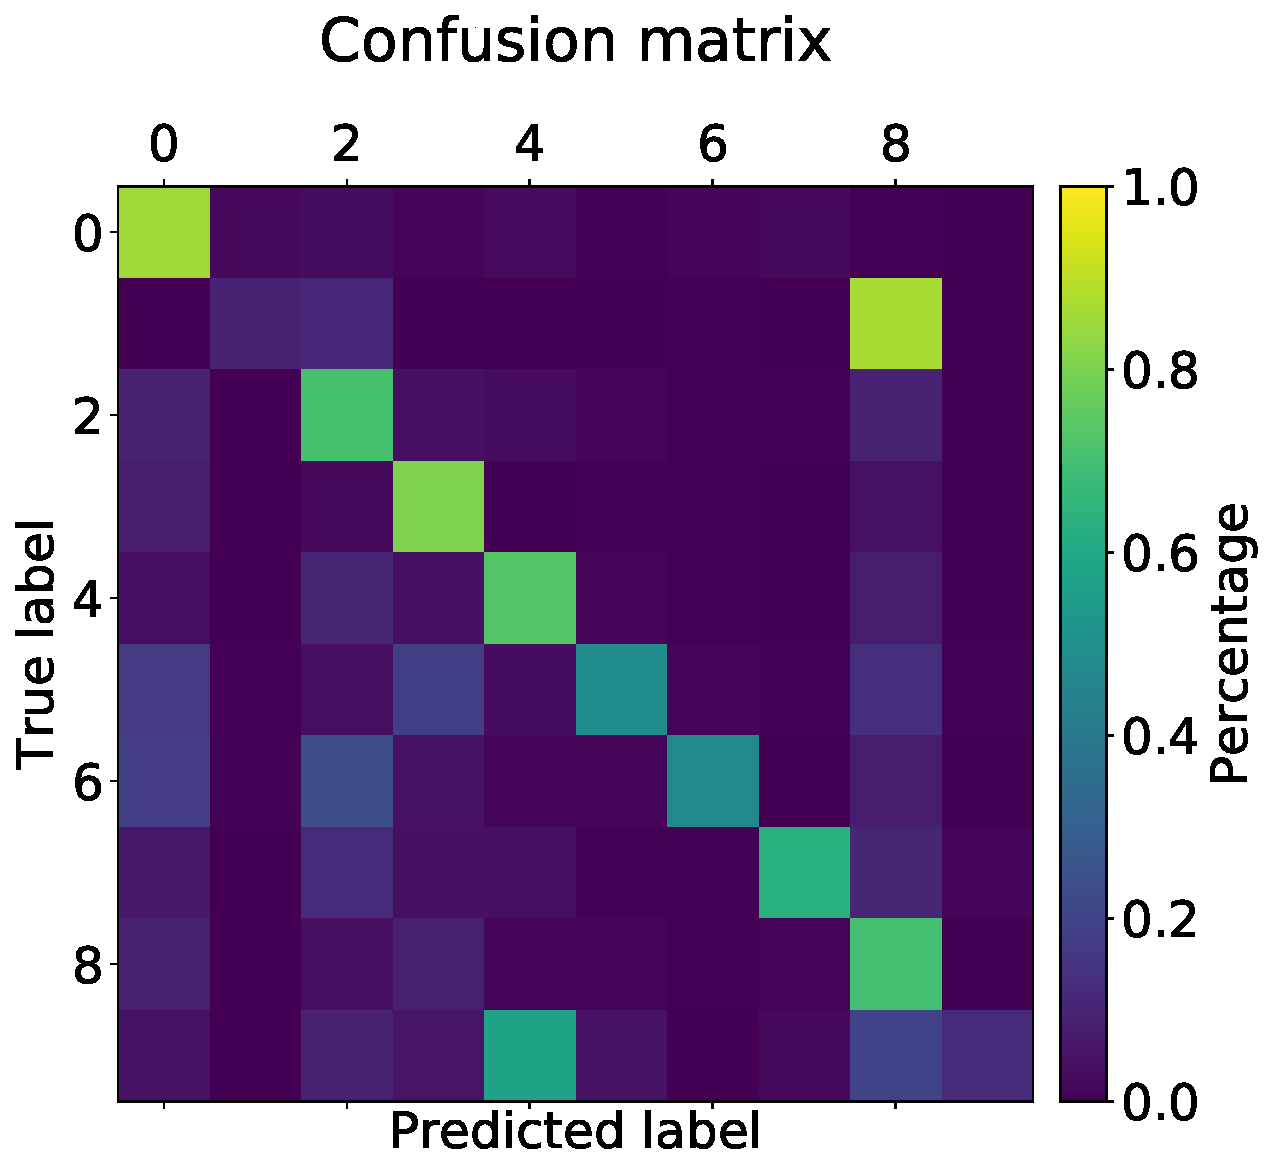
\includegraphics[width=0.30\linewidth, trim=0cm 0cm 0cm 1.5cm, clip=true]{mnist_confusion_matrix_rate_based_case_1_rate_pynn8_1dlayers_3x_20200217}&
        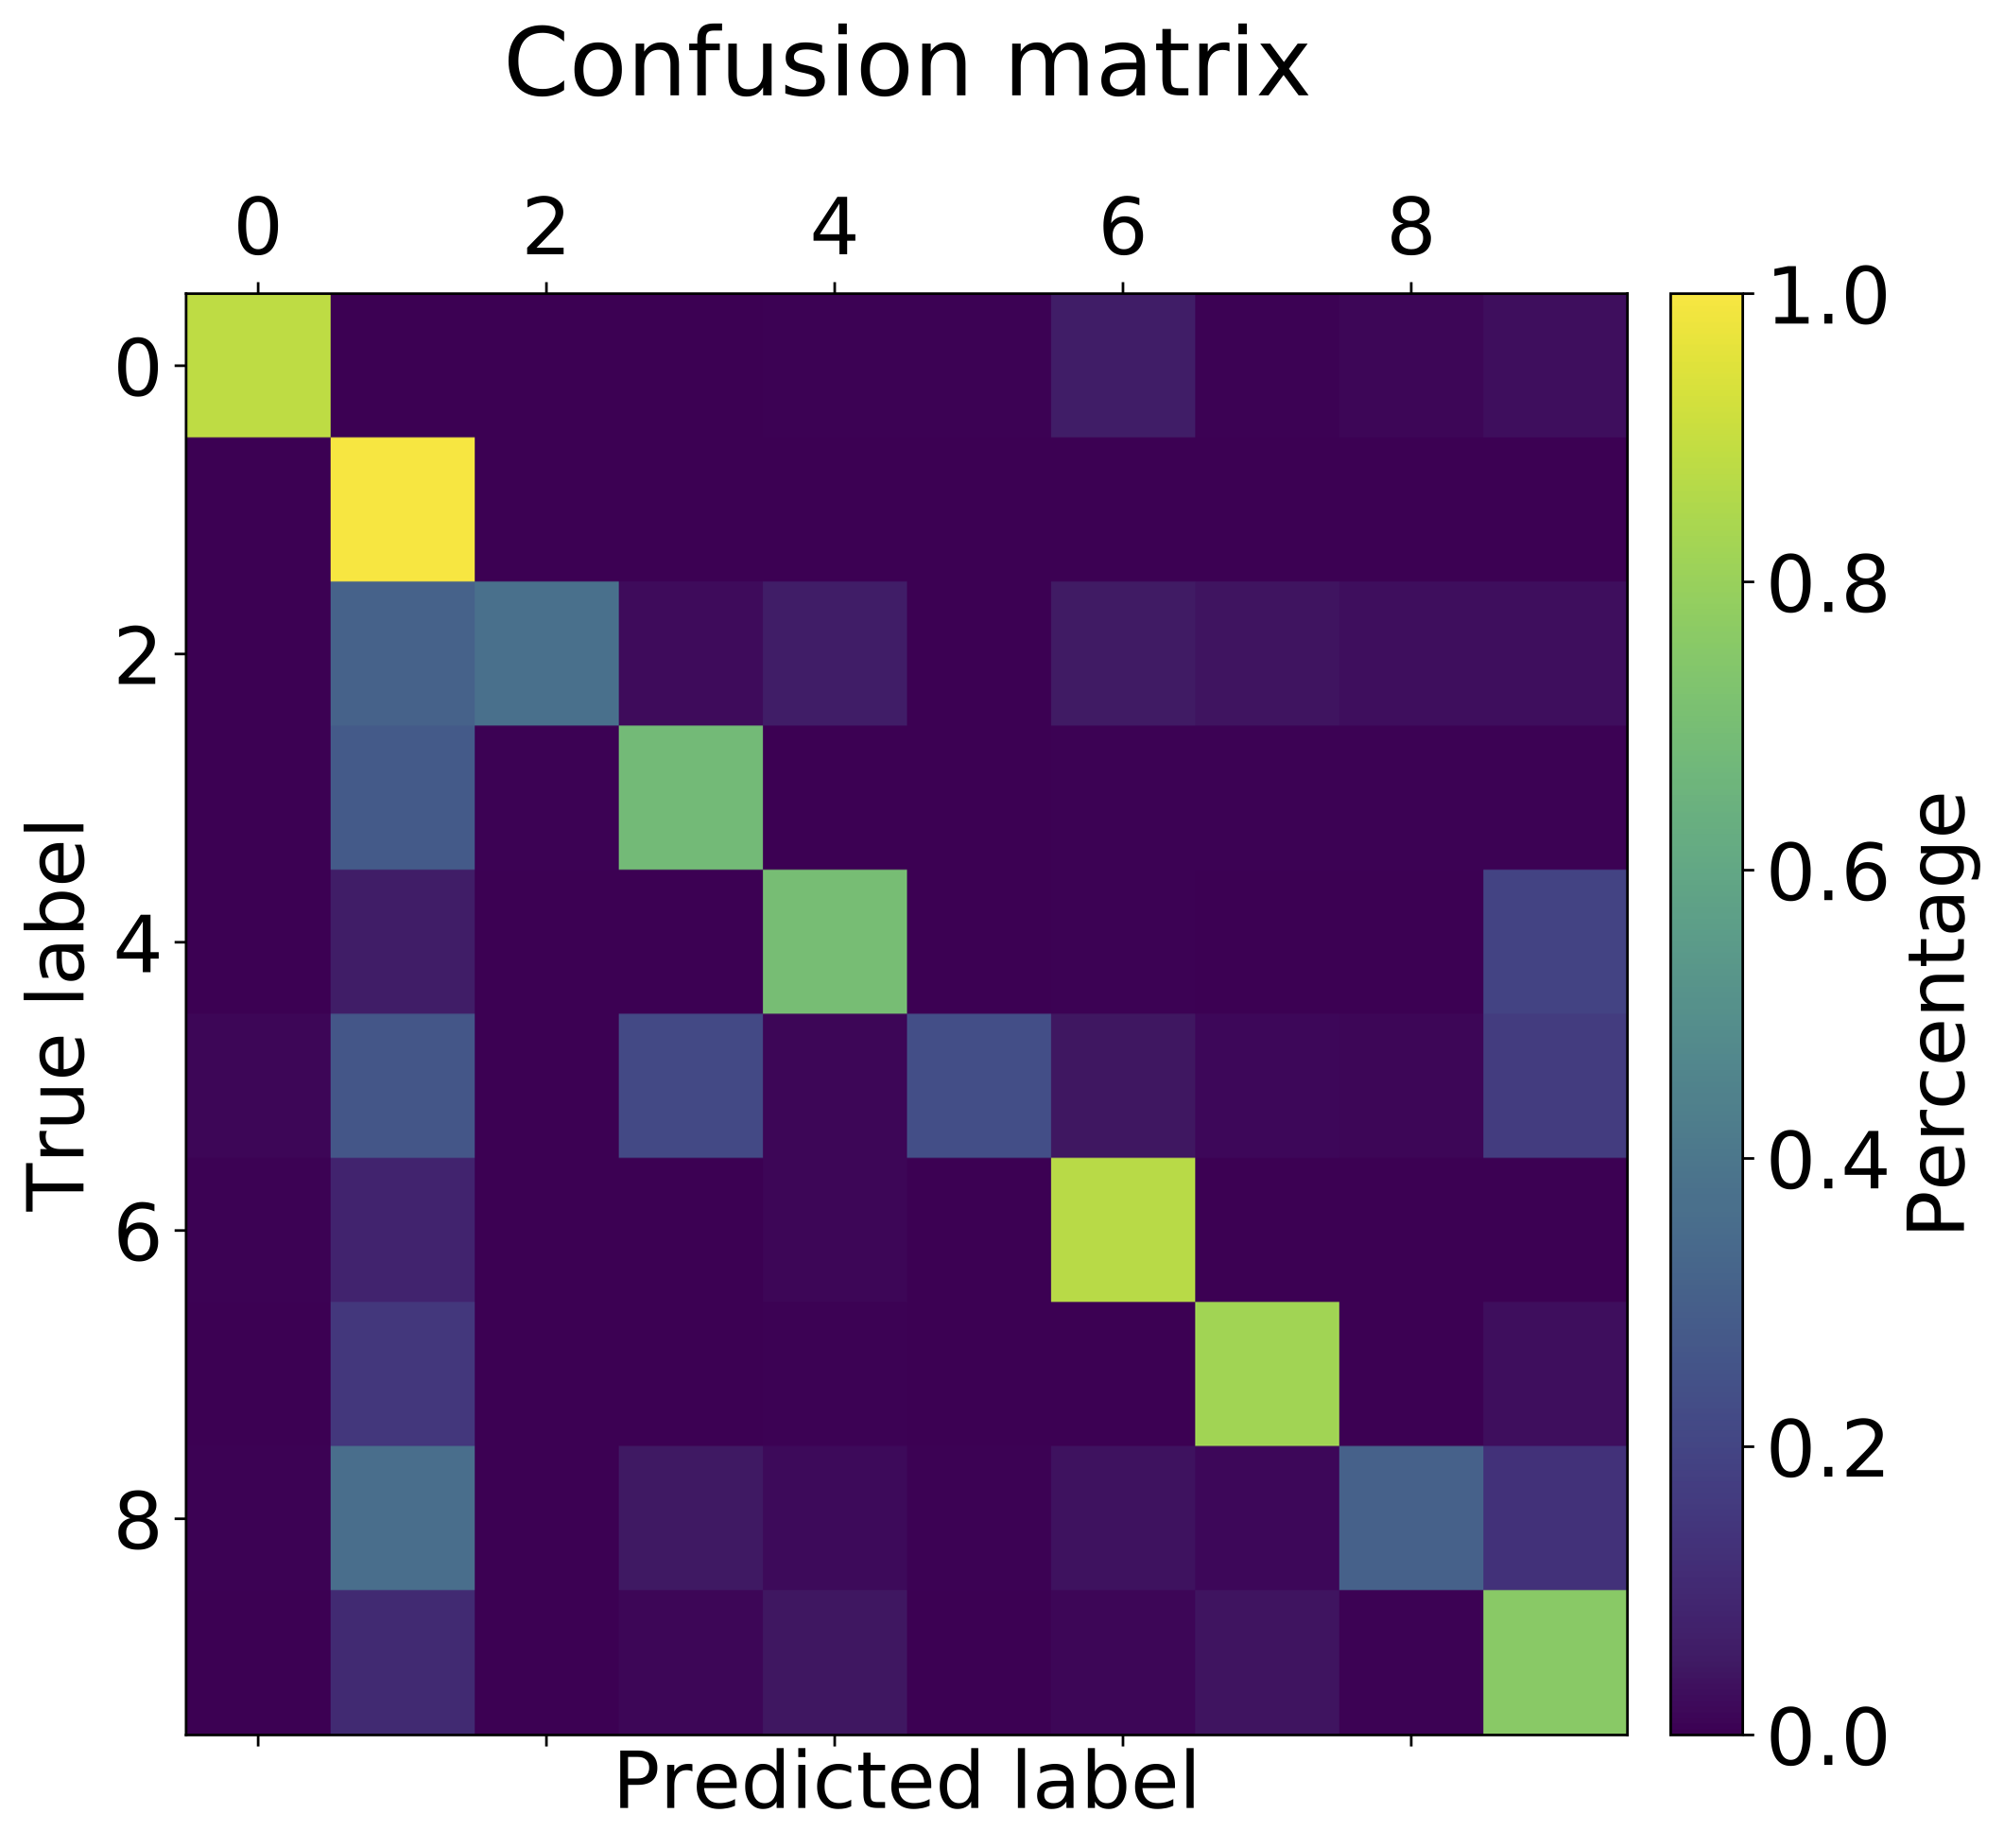
\includegraphics[width=0.30\linewidth, trim=0cm 0cm 0cm 1.5cm, clip=true]{mnist_confusion_matrix_rate_based_case_2_rate_pynn8_1dlayers_3x_20200217}&
        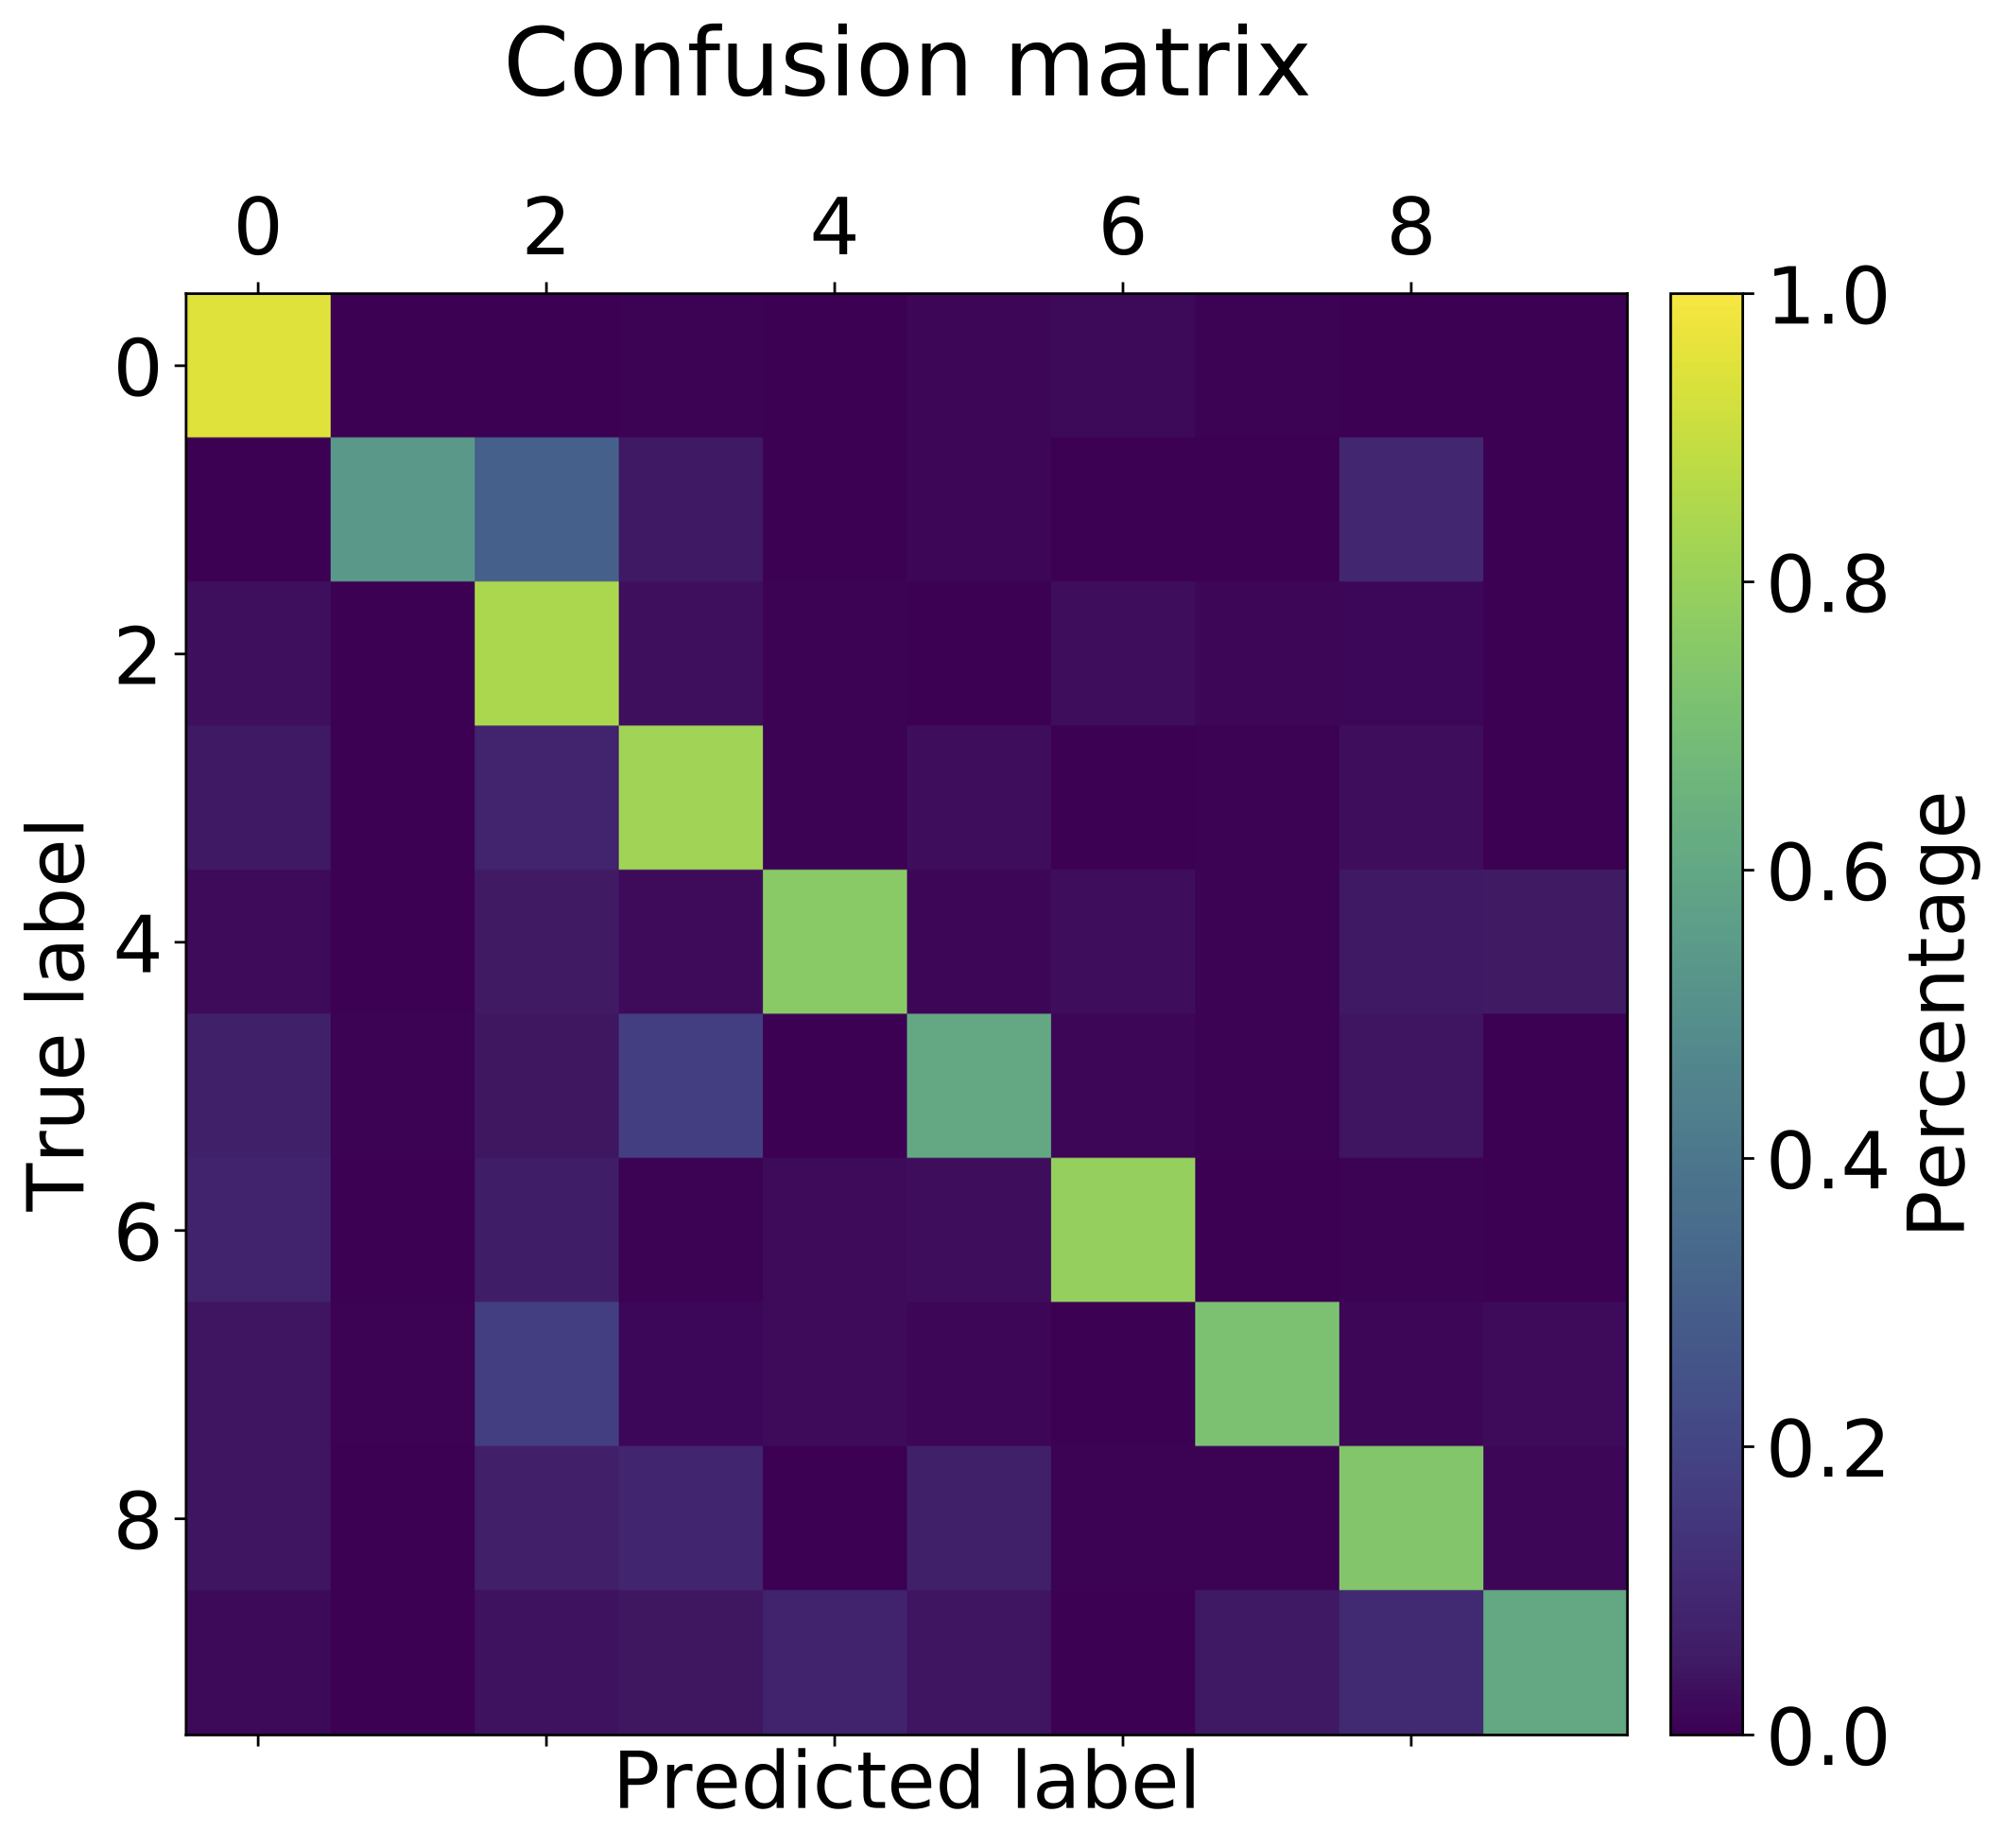
\includegraphics[width=0.30\linewidth, trim=0cm 0cm 0cm 1.5cm, clip=true]{mnist_confusion_matrix_rate_based_case_3_rate_pynn8_1dlayers_2x_20200217}\\
        Case 1, 1 hlayers & Case 2, 1 hlayers & Case 3, 1 hlayers
        \end{tabular}
     \end{centering}
     \caption{Confusion matrices for classification}
     \label{fig:confmat}
    \vspace{-10pt}
\end{figure*}

Figure \ref{fig:confmat} shows the confusion matrices which are constructed for each of the experimental cases.
When taken together with the confusion matrices, there are many misclassification of 1's from most of other classes.


One of reasons for bad performance might be that the firing rate goes down with each subsequent layer. While the firing rate of inputs is 5Hz, average firing rates of trained outputs are less than 5, as shown in Fig. \ref{fig:fr_bp_c3}. A way to keep firing rates between layers while neurons forming and removing connections needs to consider enforcing some level of  homeostasis by maintaining a target firing rate.

\begin{figure}[tbh]
    \centering
    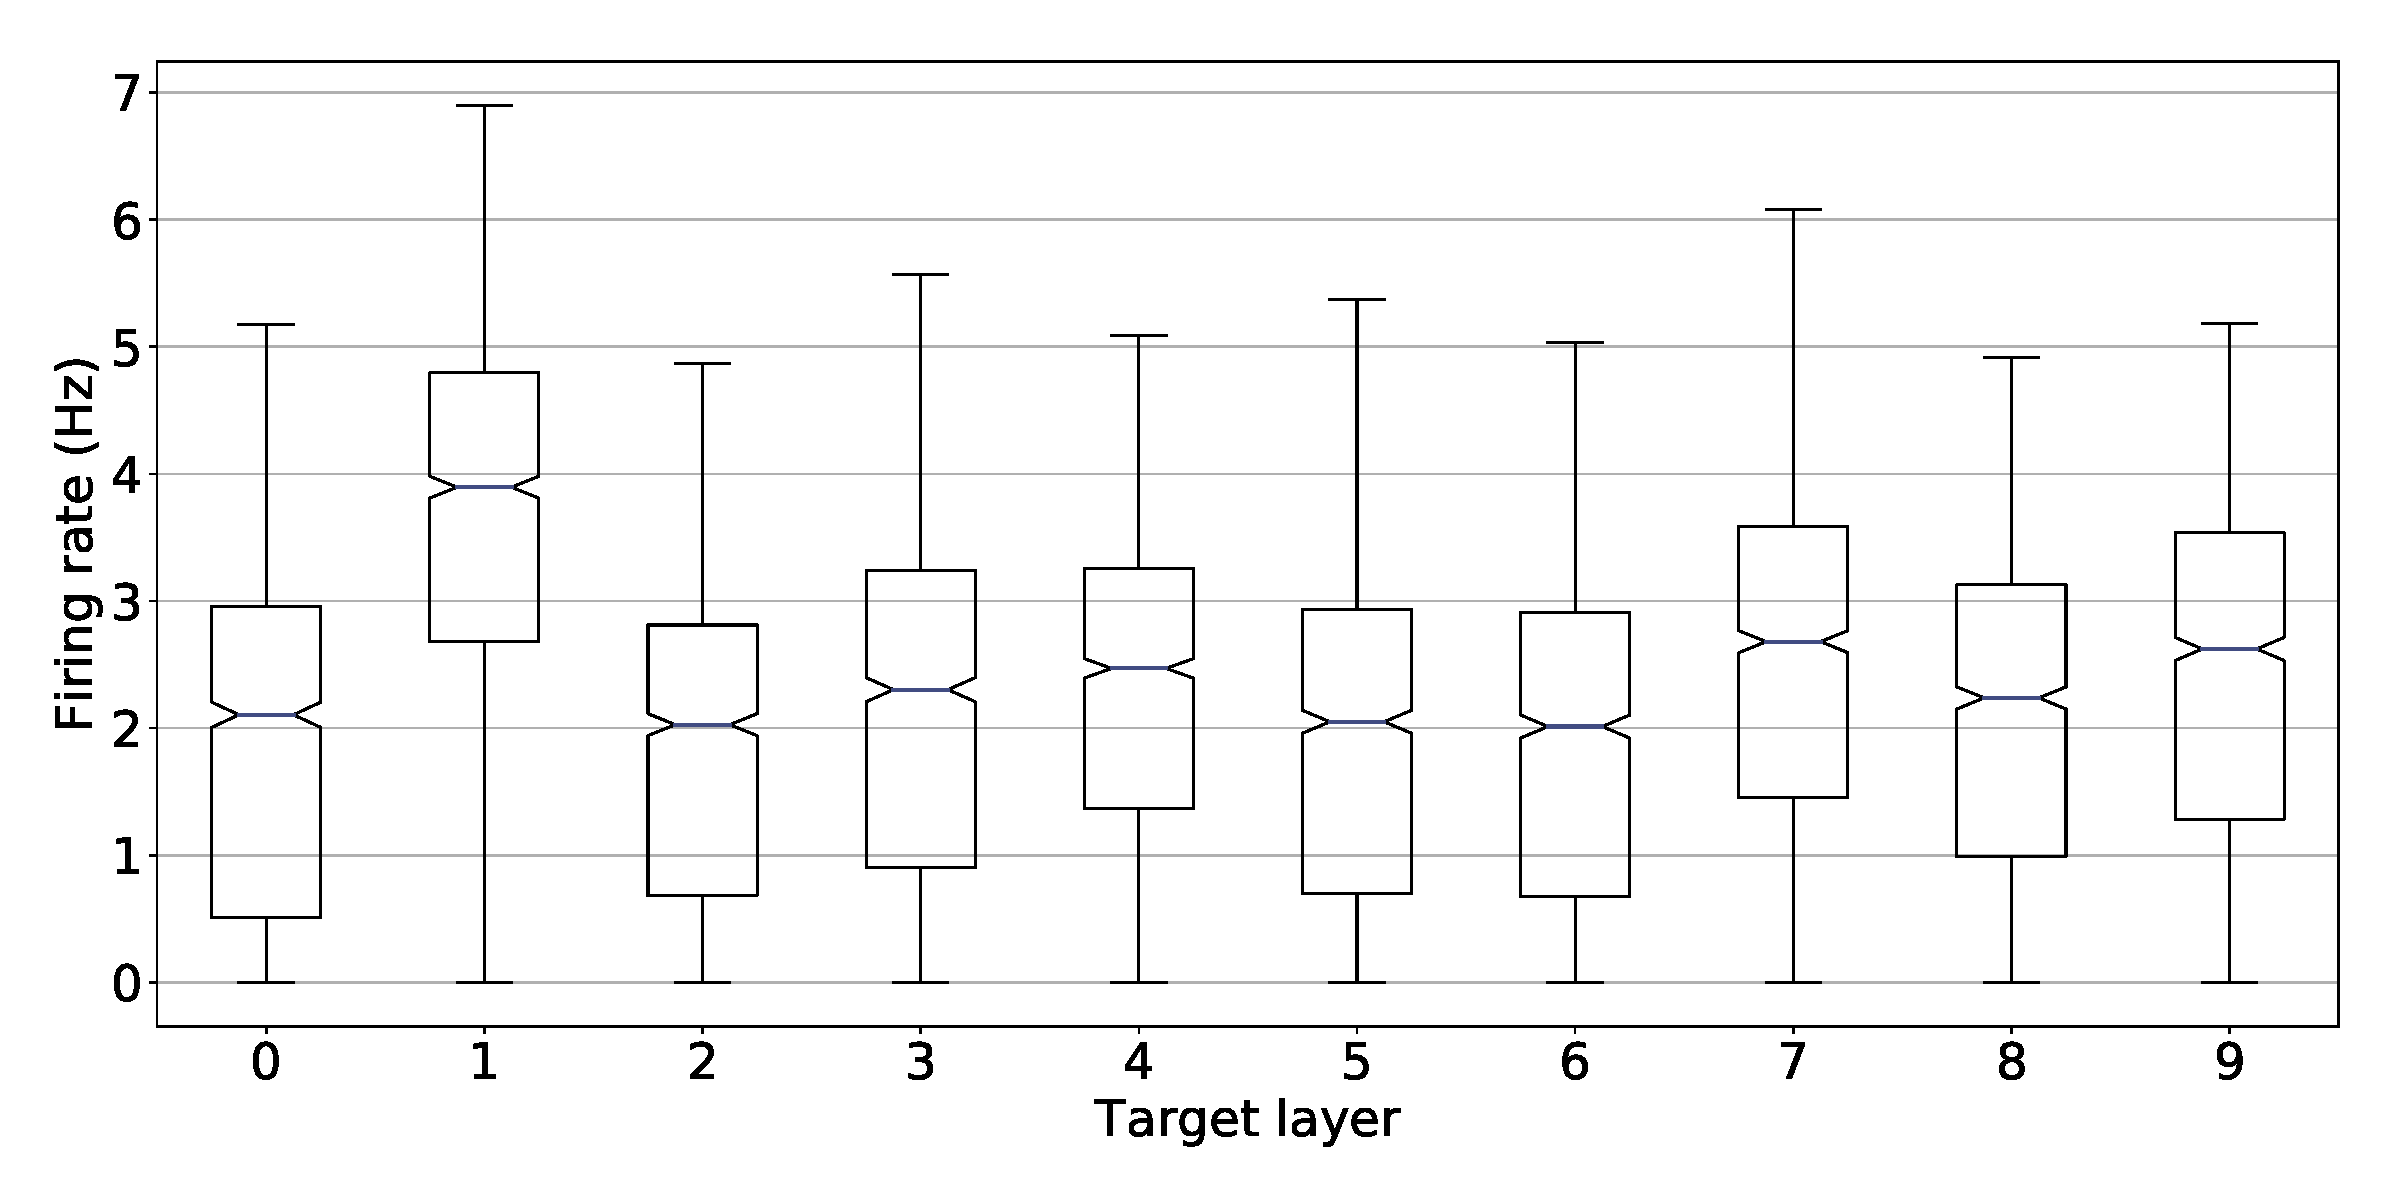
\includegraphics[width=0.80\linewidth, trim=0cm 0cm 0cm 0cm, clip=true]{mnist_training_firing_rate_boxplot_case_3_rate_pynn8}
    \caption{An example of trained firing rate for Case 3}
    \label{fig:fr_bp_c3}
\end{figure}

Additionally, excitatory feedforward connections to the next layer might play a role as Gaussian filters. They are widely used  to reduce image noise and reduce detail or make the result of blurring an image \cite{nixon2019feature}. Thus, the more hidden layers, the worse performances have been achieved even with lateral inhibitory connections.
Here, inhibitory feedforward connections can induce the effect of difference of Gaussians (DoG) with excitatory feedforward connections. DoG is a widely used effect in graphics software, typically for feature enhancement by increasing the visibility of edges and other detail. Moreover, Since Dog have also been used for scale-invariant feature detection \cite{lowe2004distinctive, bay2006surf}, it will provide opportunities to change scales between layers. 


%%-------------------------------------------------------------------------
%\section{Discussion}
%% 
%%------------------------------------------------------------------------

\section{Conclusions}\label{sec:conclusions}

In this paper, the implementation of structural plasticity on SpiNNaker has extended network depth to include multiple hidden layers. 
The proposed model has been applied for handwritten digit classification. 

There are also several areas for further development and applications.
Firstly, we have a plan to regulate network connectivity and activation  such as homeostatic plasticity \cite{Tien2018} which keeps balance of the activity level of networks because then number of connections between layers and action firing rates go down with increased depth. 
Secondly, the idea of feed-forward inhibition which is regarded capable of regulating the inhibition/excitation balance and thereby influencing the gain, the integration window, and the temporal precision of inputs \cite{DSouza2016} is considered to learn robust features. 
Beyond handwritten digit recognition, we are considering more general object recognition by combining visual attention \cite{Rea2013}.

\bibliography{strona}
\end{document}
